\documentclass[11pt]{article}

% load some asm stuff -
\usepackage{amssymb}
\usepackage{amsmath}
\usepackage{amsthm}
%\usepackage{palatino,lettrine}
\usepackage{fancyhdr}
\usepackage{epsfig}
\usepackage[round,comma,sort]{natbib}
\usepackage{simplemargins}
\usepackage{setspace}
\usepackage{wrapfig}
\usepackage{hyperref}
%\usepackage{boiboites}
\usepackage[margin=0pt,font=small,labelfont=bf]{caption}
\newcommand{\boldindex}[1]{\textbf{\hyperpage{#1}}}
\usepackage{makeidx}\makeindex
\bibliographystyle{plos2015}


\usepackage{algpseudocode}
\usepackage{algorithm}

% Set the size
%\textwidth = 6.75 in
%\textheight = 9.75 in
%\oddsidemargin = 0.0 in
%\evensidemargin = 0.0 in
%\topmargin = 0.01 in
%\headheight = 0.0 in
%\headsep = 0.25 in
%\parskip = 0.15in
% \doublespace
\setallmargins{1in}

\newtheorem{example}{Example}[section]
\newtheorem{thm}{Theorem}[section]
\newtheorem{property}{Property}[section]

\theoremstyle{definition}
\newtheorem{defn}[thm]{Definition}

\makeatletter
% \renewcommand\subsection{\@startsection
% 	{subsection}{2}{0mm}
% 	{-0.05in}
% 	{0.1\baselineskip}
% 	{\normalfont\normalsize\bfseries}}
\renewcommand\subsubsection{\@startsection
	{subsubsection}{2}{0mm}
	{-0.05in}
	{-0.5\baselineskip}
	{\normalfont\normalsize\itshape\bfseries}}
\renewcommand\paragraph{\@startsection
	{paragraph}{2}{0mm}
	{-0.05in}
	{-0.5\baselineskip}
	{\normalfont\normalsize\itshape}}
\makeatother
\linespread{1.1}

\fancypagestyle{proposal}{\fancyhf{}%
	\fancyhead[RO,LE]{\thepage}%
	\fancyhead[LO,RE]{CHEME 131 Module 3 STRIPS}%
	\renewcommand\headrulewidth{1pt}}
\pagestyle{proposal}

\usepackage{mdframed}
\definecolor{lgray}{rgb}{0.92,0.92,0.92}
\definecolor{antiquewhite}{rgb}{0.98,0.92,0.84}
\definecolor{lightskyblue}{rgb}{0.93,0.95,0.99}

% defn environment
\mdfdefinestyle{theoremstyle}{% 
    linecolor=black,linewidth=1pt,% 
    frametitlerule=true,% 
    frametitlebackgroundcolor=lgray, 
    innertopmargin=\topskip,} 
\mdtheorem[style=theoremstyle]{definition}{Definition}

% concept environment
\mdfdefinestyle{conceptstyle}{% 
    linecolor=black,linewidth=1pt,% 
    frametitlerule=true,% 
    frametitlebackgroundcolor=lightskyblue, 
    innertopmargin=\topskip,} 
\mdtheorem[style=conceptstyle]{concept}{Concept}
\newcommand{\newterm}[1]{{\it #1}}

% Single space'd bib -
\setlength\bibsep{0pt}

\renewcommand{\rmdefault}{phv}\renewcommand{\sfdefault}{phv}
%\newboxedtheorem[boxcolor=black, background=gray!5,titlebackground=orange!20,titleboxcolor = black]{color_box_example}{Example}{test}

% Change the number format in the ref list -
\renewcommand{\bibnumfmt}[1]{#1.}

% Change Figure to Fig.
\renewcommand{\figurename}{Fig.}
\usepackage{enumitem}
\setlist{noitemsep} % or \setlist{noitemsep} to leave space around whole list

%Joycelyn Chan, Joshua Lequieu, Michael Paull, Chidanand Balaji, Ryan Tasseff
%Our derivation follows closely the earlier development of Fredrickson \citep{Fredrickson:1976fk}.

% Begin ...
\begin{document}

%\begin{titlepage}
{\par\centering\textbf{\Large CHEME 131 Module 3: Registered Interest and Principal of Securities (STRIPS) Bonds}}
\vspace{0.2in}
{\par \centering \large{Jeffrey D. Varner}}
\vspace{0.05in}
{\par \centering \large{Smith School of Chemical and Biomolecular Engineering}}
{\par \centering \large{Cornell University, Ithaca NY 14853}}
% \vspace{0.1in}
% {\par \centering \small{Copyright \copyright\ Jeffrey Varner 2018. All Rights Reserved.}}\\

%\end{titlepage}
\date{}
\thispagestyle{empty}

\setcounter{page}{1}

\section*{Introduction}
\href{https://en.wikipedia.org/wiki/United_States_Treasury_security#STRIPS}{Registered Interest and Principal of Securities (STRIPS) bonds} are a 
unique type of fixed-income investment instrument that provides investors with an alternative way to access the coupon payments of 
Treasury securities. STRIPS bonds are created by separating a Treasury securities coupon and principal components and trading them as individual 
zero-coupon securities. This process allows investors to purchase and trade the coupon or principal components separately, 
providing greater flexibility in managing their investment portfolios.

\begin{figure}[h]
    \centering
    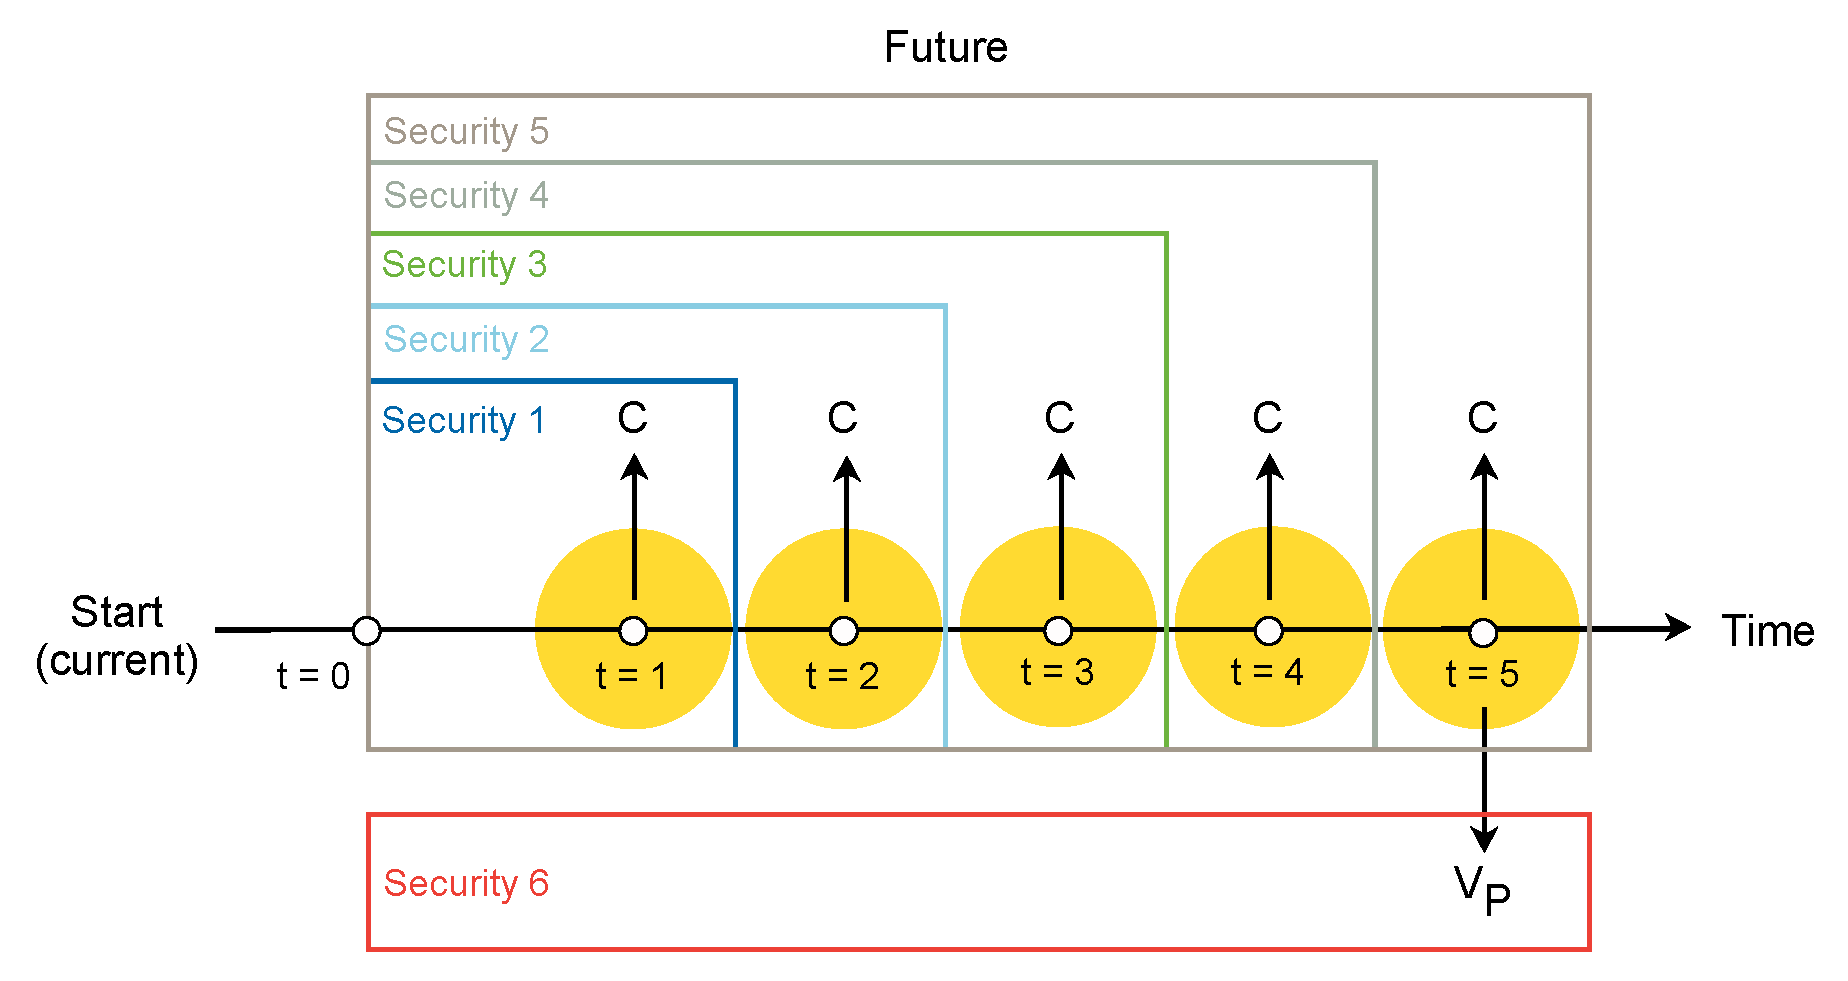
\includegraphics[width=0.85\textwidth]{./figs/Fig-STRIPS-Schematic.pdf}
    \caption{Schematic of a Registered Interest and Principal of Securities (STRIPS) bond generated from a 5-year Treasury note. The coupon and principle payments from the coupon-based 
	note are stripped fron the original instrument and sold as seperate marketable securities.}\label{fig:strips-bond-schematic}
\end{figure}

For example, a 5-year Treasury note with annual coupon payments of $C$ USD and a face (par) value of $V_{P}$ (USD)
can be stripped into six separate zero-coupon securities, i.e., five zero-coupon bonds, each with face values of $C$ 
and maturity of $T$= 1,2,3,4 and 5 years, and a six security with face  (par) value of $V_{P}$ USD with a duration of $T$ = 5 years (Fig. \ref{fig:strips-bond-schematic}). 
In the general case, a treasury note or bond with $N=\lambda{T}$ coupon payments, where $T$ denotes the maturity in years, and $\lambda$ represents 
the number of coupon payments per year, can be stripped into $N+1$ separate zero-coupon securities.
Beyond thier immediate value as investment tools, STRIPS are interesting as they provide look at the 
\href{https://www.federalreserve.gov/data/yield-curve-models.htm}{term structure of interest rates}, i.e., the relationship between the remaining time-to-maturity of debt securities 
and the yield on those securities.

In this module, we'll explore the mathematics of STRIPS bonds, and how they can be used to understand the term structure of interest rates, 
i.e., how we can use STRIPS to compute the short-rates, and the yield curve.

\end{document}
